% Advisor meeting brief (to share): the three most important results since the residual-stream discussion, with
% figures and the questions to decide. Numbers follow exp4/LOG.md and exp5/LOG.md (independently verified wording).
% Figures: exp4b_heads.png (exp4/onepager_capital_figures.py), meet_exp5.png (exp5/meeting_figures.py).
% Build (from this folder): pdflatex advisor_brief_2026-11-03.tex
\documentclass[10pt]{article}
\usepackage[letterpaper,hmargin=0.55in,vmargin=0.32in]{geometry}
\usepackage[T1]{fontenc}
\usepackage[scaled=0.92]{helvet}
\renewcommand{\familydefault}{\sfdefault}
\usepackage{microtype}
\usepackage{xcolor}
\usepackage{graphicx}
\usepackage{enumitem}
\usepackage[hidelinks]{hyperref}
\setlength{\parindent}{0pt}
\setlength{\parskip}{2pt}
\setlist{nosep,leftmargin=1.2em,itemsep=1.5pt}
\definecolor{cblue}{HTML}{2A78D6}
\definecolor{ink2}{HTML}{52514E}
\definecolor{muted}{HTML}{898781}
\definecolor{plane}{HTML}{F4F3EF}
\newcommand{\res}[2]{\par\vspace{5pt}{\large\bfseries\color{cblue}#1}\ {\large\bfseries #2}\\[-3pt]\rule{\linewidth}{0.5pt}\par}

\begin{document}

{\LARGE\bfseries Where the ``no-op'' lives: three results}\\[2pt]
{\small\color{ink2} GPT-2 small. Random-token rows with a country at position $\tau$ and its capital (or a wrong capital)
as the final token $T$. Each pair of sequences differs at one position only. 200 / 100 rows $\times$ 11
country--capital pairs per filler type. Every analysis was pre-registered and independently re-checked.}

\res{1}{The matching capital lowers late resting at every distance, through specific head families}
{\centering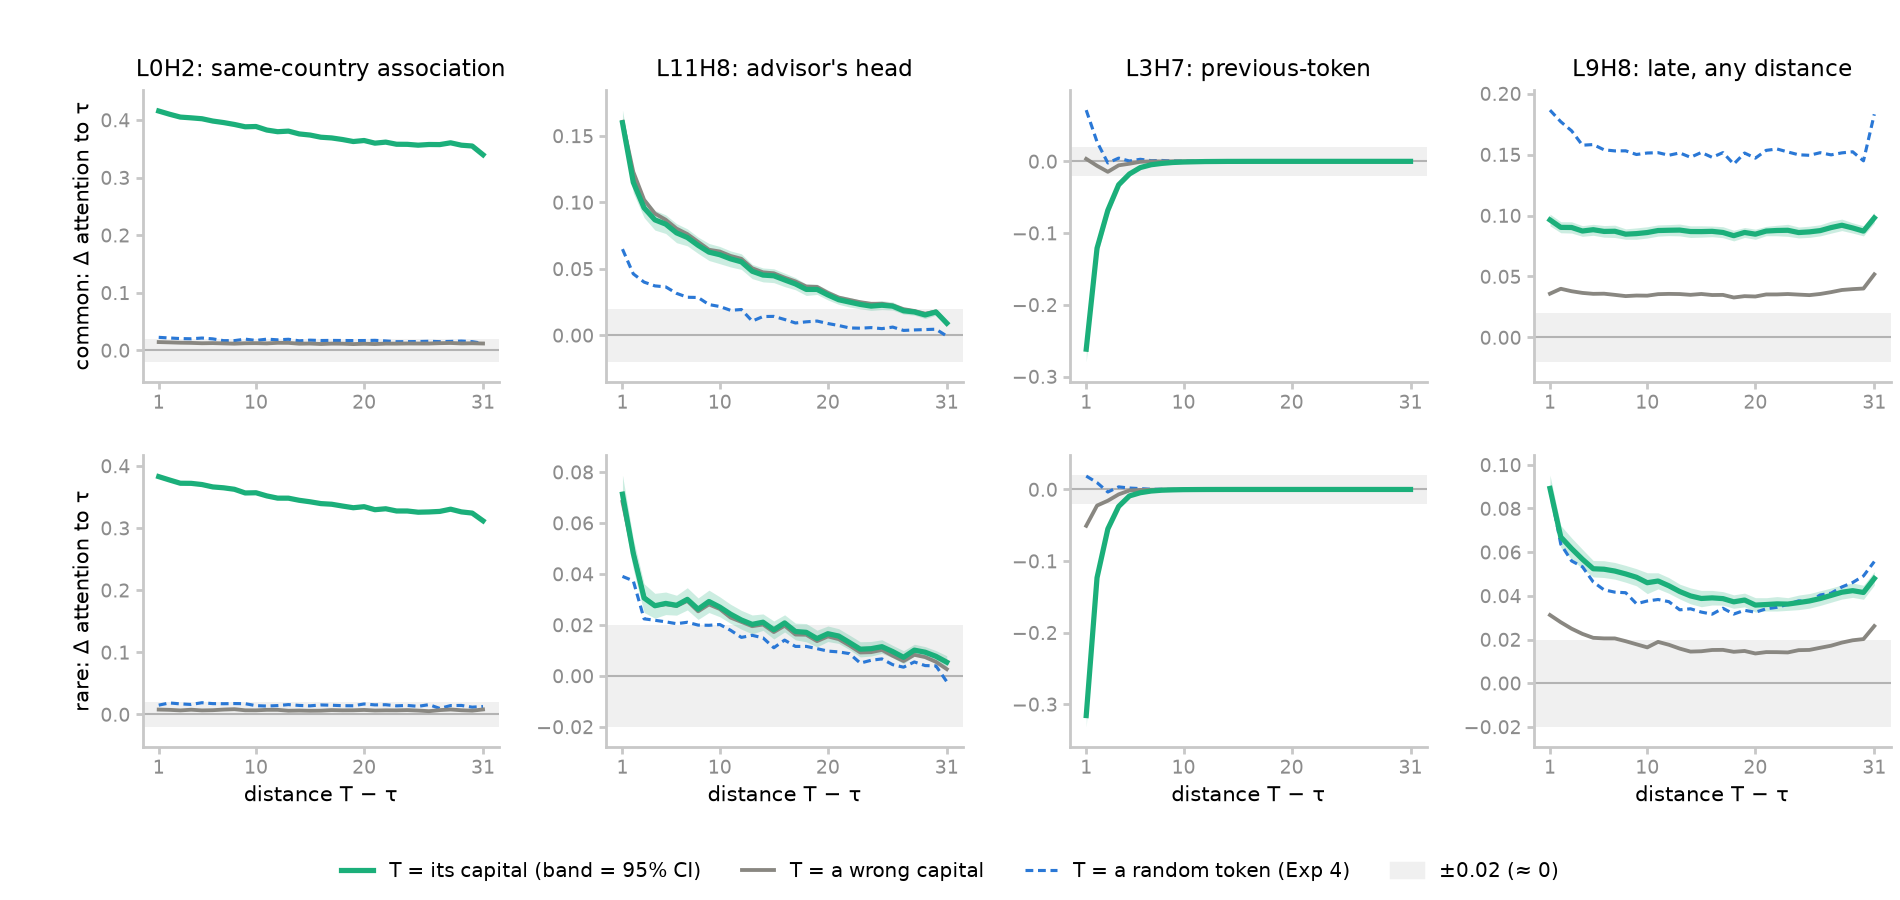
\includegraphics[width=0.56\linewidth]{exp4b_heads.png}\par}
\begin{itemize}
\item Late-layer attention parked on BOS drops by \textbf{0.02--0.04} with the country's own capital at $T$, against a
  wrong capital, at every distance from 1 to 31 tokens. A placebo word at $\tau$ gives $\approx 0$.
\item \textbf{Same-country heads from layer 0.} L0H2 gives the country 0.43 of its attention with its own capital and
  0.03 with a wrong one. L4H10, L3H0 and L1H11 do the same, but for any same-country pair (demonyms, cities), not
  specifically ``capital of''.
\item The advisor's L11H8 is not a previous-token head: it puts only 6--8\% on the previous token. Only L4H11 is a pure
  previous-token head.
\end{itemize}

\res{2}{In the residual stream, the match enters at layer 1 and the resting effect is assembled in layers 3--7}
{\centering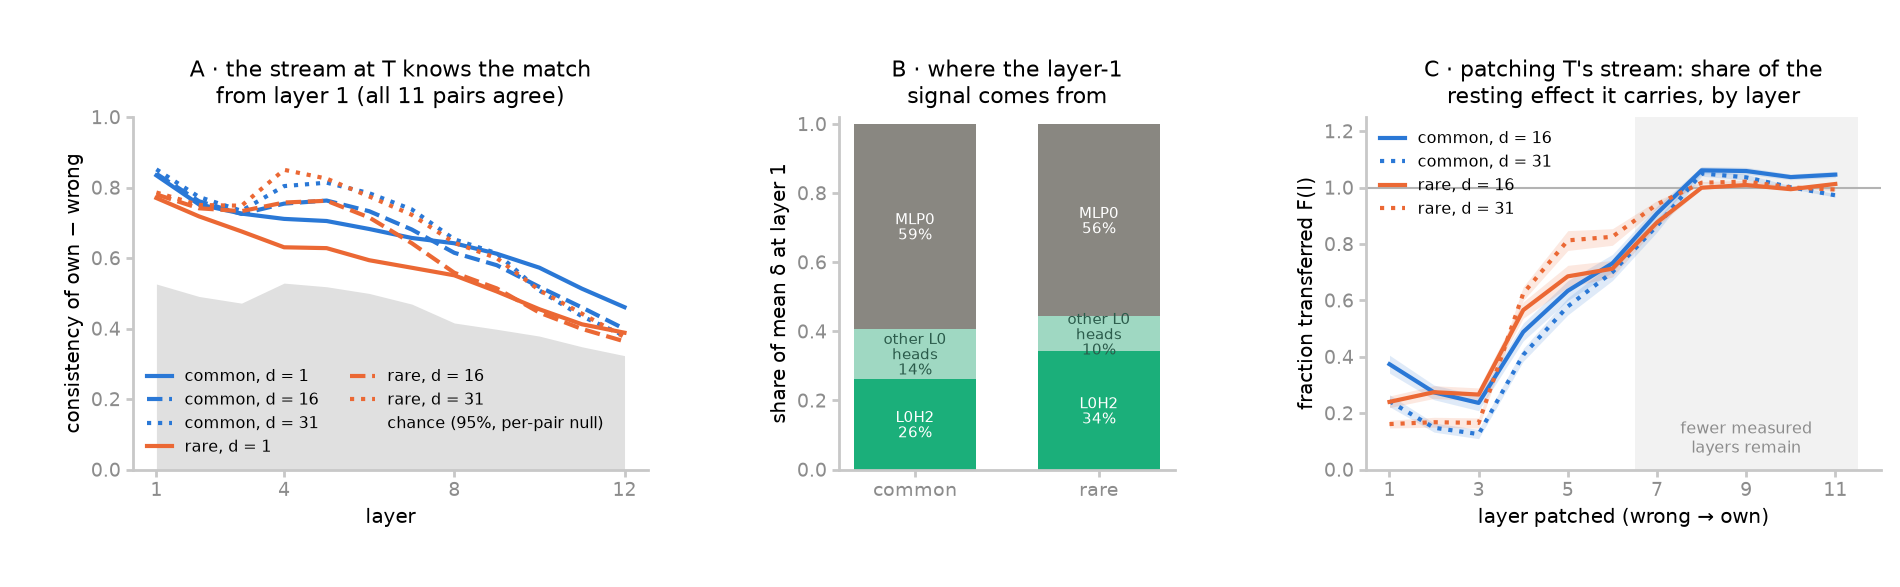
\includegraphics[width=0.92\linewidth]{meet_exp5.png}\par}
\begin{itemize}
\item \textbf{A.} From layer 1, the stream at $T$ carries an own-vs-wrong direction shared by all 11 pairs (exact
  per-pair null $p = 1/1024$ at every layer, margin 1.3--1.6$\times$).
\item \textbf{B.} At layer 1 it comes from L0H2 (26--34\%), the other layer-0 heads (10--14\%) and the first MLP
  (56--59\%). It is a ``matching country attended'' signal, not the country's identity: a mismatched country looks
  like filler to $T$.
\item \textbf{C.} Patching: $T$'s stream carries 12--37\% of the resting effect by layer 3, a step at layer 4, and
  86--94\% by layer 7. From layer 8 it reproduces the effect within $\pm 6\%$. Context still matters at layers 6--7.
\end{itemize}

\res{3}{In the writes, ``no-op'' means a constant offset}
Heads that rest on BOS write less varied vectors ($\rho = -0.67$ / $-0.70$ across 144 heads). But the BOS term is
effectively a fixed vector, about 2\% of write variance, and per unit of attention \emph{not} on BOS resting heads
write as much variety as active heads or more. So the no-op is attention reweighted onto a constant, not quieter
reading.

\vspace{2pt}
{\small\color{ink2}\textbf{Did not hold:} distance dependence falling with depth (it rises); clean topological clusters
of heads; the four same-country heads carrying $\ge$20\% of the patching effect (18--36\%, fragile).}

\vspace{5pt}
\colorbox{plane}{\parbox{\dimexpr\linewidth-2\fboxsep}{\small
\textbf{The main caveat.} Everything rests on the same 11 country--capital pairs. In paired tests the effective $n$
is 11, so ``beyond the null'' means consistent across rows, not general.\\[3pt]
\textbf{To decide together}
\begin{enumerate}[leftmargin=1.4em]
\item Generalise first (more countries; cities and demonyms at $\tau$ to separate ``capital of'' from same-country
  relatedness), or go deeper (the first MLP's 56--59\%; the layer 3--7 assembly)?
\item Is ``no-op = attention reweighted onto a constant BOS vector'' the right claim to build on?
\end{enumerate}}}

\end{document}
